\chapter{Conclusions} \label{ch:conclusions}

\section{Summary of findings}

Transcription factor-DNA interactions \textit{in vivo} are the fundamental events in the regulatory network of transcription. The interrogation of genome-wide binding events of three Forkhead transcription factors presented in this study demonstrates that the DNA binding of a transcription factor in a living cell involves great subtleties.

FOXM1 does not bind to the canonical Forkhead consensus \textit{in vivo}, although specific interactions between FOXM1 and the Forkhead consensus can be observed \textit{in vitro} at a low affinity. Instead, the chromatin recruitment of FOXM1 needs the presence of the MMB complex. It cooperates with the MMB complex to occupy the promoters of a large array of genes whose transcriptional activities peak at the G2 and M phases. Therefore, FOXM1 gains its own specific binding events and unique functions in the regulation of the mitosis relative to other Forkhead proteins by interacting with the MMB complex. These findings reinforce the notion that the protein-protein interaction plays an essential role in the achievement of specific binding events of a transcription factor \textit{in vivo}.

FOXK2 and FOXO3 bind to both specific and shared regions in the genome, and the majority of the FOXO3 binding events are shared with FOXK2. Both factors bind to the Forkhead consensus \textit{in vitro} and \textit{in vivo}, but sequence preferences at the positions flanking the Forkhead consensus partially dictate the specific binding sites of FOXK2, which strengthens previous findings that nucleotides flanking the core consensus are important for the specificity among family members (\cite{wei2010genome-wide}). Furthermore, different TF-TF interactions also possibly contribute to the specific binding events of FOXK2 and FOXO3. In addition, neither competitive nor assisted binding can be observed between the binding of FOXK2 and FOXO3 on their shared binding regions, indicating that their binding at those regions might be highly dynamic.

Based on the results presented in this study, we propose the following models for the \textit{in vivo} DNA-binding events of FOXM1, FOXK2 and FOXO3: under normal condition when PI3K/AKT pathway is active, FOXO3 is sequestered in the cytoplasm; FOXM1 and FOXK2 are in the nucleus, but FOXM1 is unable to compete with FOXK2 to bind the Forkhead consensus; instead, FOXM1 occupies the promoters where the CHR motif is located by interacting with the MMB complex, and this MMB/FOXM1 complex plays a critical role in the transcriptional regulations of the genes whose activities peak at the G2 and M phases (\textbf{Figure \ref{fig:fig56}}, top panel); when the PI3K/AKT pathway is inhibited, FOXO3 enters into the nucleus and mostly binds to regions where FOXK2 is located, but the relationship between the binding of FOXK2 and FOXO3 remains unknown (\textbf{Figure \ref{fig:fig56}}, bottom panel).

\begin{figure}[!h]
    \centering
    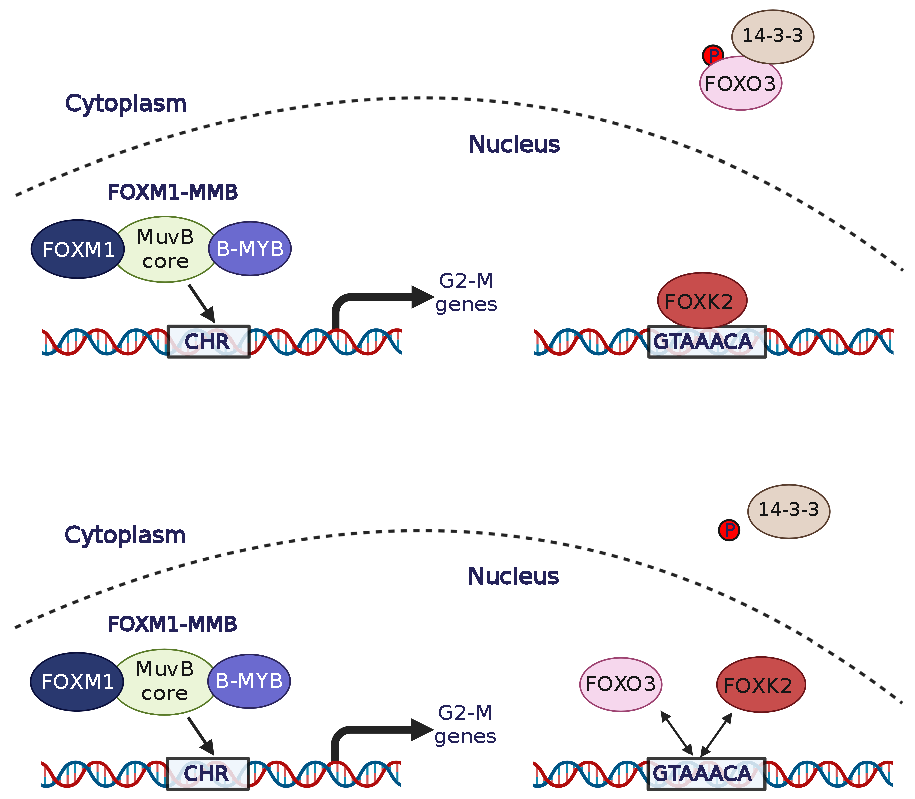
\includegraphics[width=0.9\textwidth]{chapter5/figures/fig56.pdf}
    \caption[Models for the DNA-binding events of FOXM1, FOXK2 and FOXO3 \textit{in vivo}]{\textbf{Models for the DNA-binding events of FOXM1, FOXK2 and FOXO3 \textit{in vivo}.} See the main text for detailed description. The dotted line represents the nuclear envelope.}
    \label{fig:fig56}
\end{figure}

\section{Unanswered questions and future work}

\subsection{Does FOXM1 directly contact DNA \textit{in vivo}?}

Since formaldehyde can crosslink both protein-DNA and protein-protein interactions, a binding event of a transcription factor detected by ChIP experiments can be due to both direct and indirect DNA contacts. It is impossible to tell whether a protein really directly contacts DNA using ChIP experiments. However, if a consensus motif is present around the summit of a transcription factor binding site, one tends to believe that it is a direct contact. Unfortunately, this is not the case in the FOXM1 cistrome. We do notice that some FOXM1 binding events do not overlap with either LIN9 or B-MYB, indicating that some chromatin binding events of FOXM1 are probably independent of the MMB complex. Therefore, it is still possible that FOXM1 directly contact DNA or is recruited by another factor. Motif discovery is supposed to shed some light on this, but this analysis only returns the CCAAT-box motif, the CHR motif and a GC-rich motif. It is possible that some zinc-finger proteins, which bind to the GC-rich sequence, recruit FOXM1 to the chromatin of the promoters at a subset of its target genes, or that FOXM1 binds to a very short DNA element which contains little information content that cannot be discovered by motif analysis. Therefore, it is necessary to utilise high resolution ChIP-exo (\cite{rhee2011comprehensive}) to reveal the exact crosslinking point of FOXM1 or the proteins recruiting FOXM1 to the chromatin, which might help elucidate how FOXM1 is recruited to the chromatin.

\subsection{What is the intrinsic DNA binding specificity of FOXK2 and FOXO3?}

ChIP-seq analyses of FOXK2 and FOXO3 demonstrate that both factors can bind to the Forkhead consensus. There are no discernible preferences within the core consensus, but FOXK2 favours the sequence WWGTAAACAWS. However, the sequence motif returned by the ChIP-seq data is biased by the non-random nature of the genome, and it does not reflect the intrinsic specificity of a factor. Although bandshift experiments suggest that the nucleotides flanking the Forkhead consensus do affect the binding of FOXK2, this method is only at a low-throughput level. Therefore, to systematically investigate the intrinsic DNA binding specificity of FOXK2 and FOXO3, in vitro methods such as PBM or HT- SELEX can be used. The comparison between results from ChIP-seq and PBM/HT- SELEX of FOXK2 and FOXO3 could be very informative.

\subsection{What is the relationship of the DNA binding between FOXK2 and FOXO3 at their shared binding regions?}

Since the change of FOXK2 binding does not affect the binding of FOXO3 at the shared binding regions and vice versa, it is difficult to draw a conclusion about the relationship between DNA binding of FOXK2 and FOXO3. So far, all the experiments are done within 24 - 48 hours after the depletion of FOXK2 or the overexpression of FOXO3. It is possible that this time frame is too soon to see any effect, and that longer depletion or overexpression might help to uncover the relationship of the binding between these two factors. However, current ChIP experiments detect the steady-state binding of a factor across a population of cells. FOXK2 and FOXO3 might occupy the same locus but in different cells, and the general occupancy detected by ChIP is only a fraction of the cells. If the model proposed in \textbf{Figure \ref{fig:fig55}} is true, current ChIP technique will never catch such dynamic changes of binding. Therefore, other methods based on fluorescent microscopy like FRET or FRAP which can study protein-DNA interaction in a single cell might help to elucidate this question, but this will not allow the investigation at a single gene locus level. In addition, it is still possible that FOXK2 and FOXO3 bind to different sites within the shared peaks, which cannot be discriminated by the current resolution of sonication-based ChIP-seq. Therefore, it is necessary to perform ChIP-reChIP experiments to investigate whether FOXK2 and FOXO3 co-associate on chromatin in the same cell. High resolution ChIP-exo will also help to reveal the exact binding sites of FOXK2 and FOXO3.

\subsection{How are the binding events of FOXO3 linked to its biological functions?}

Linking the binding events of a transcription factor to its functions is critical for understanding the biological meanings of transcription factor-DNA interactions \textit{in vivo}. Extracting biological meanings from only one experiment can be dangerous, considering the dynamic nature of the TF-DNA interactions \textit{in vivo}. Therefore, in order to investigate the functions of the FOXO3 binding events, a repeat of FOXO3 ChIP-seq experiment needs to be done. Furthermore, to understand how functional specificity is achieved by FOXK2 and FOXO3, it is necessary to use gene expression arrays to find out the FOXO3-regulated genes, and make comparisons to the FOXK2-regulated genes (\cite{ji2012the}).